%-----------------------------------------------------------------------------------------------------------------------------------
\chapter{Moti relativi}
%-----------------------------------------------------------------------------------------------------------------------------------
\begin{figure}[htbp]
\begin{center}
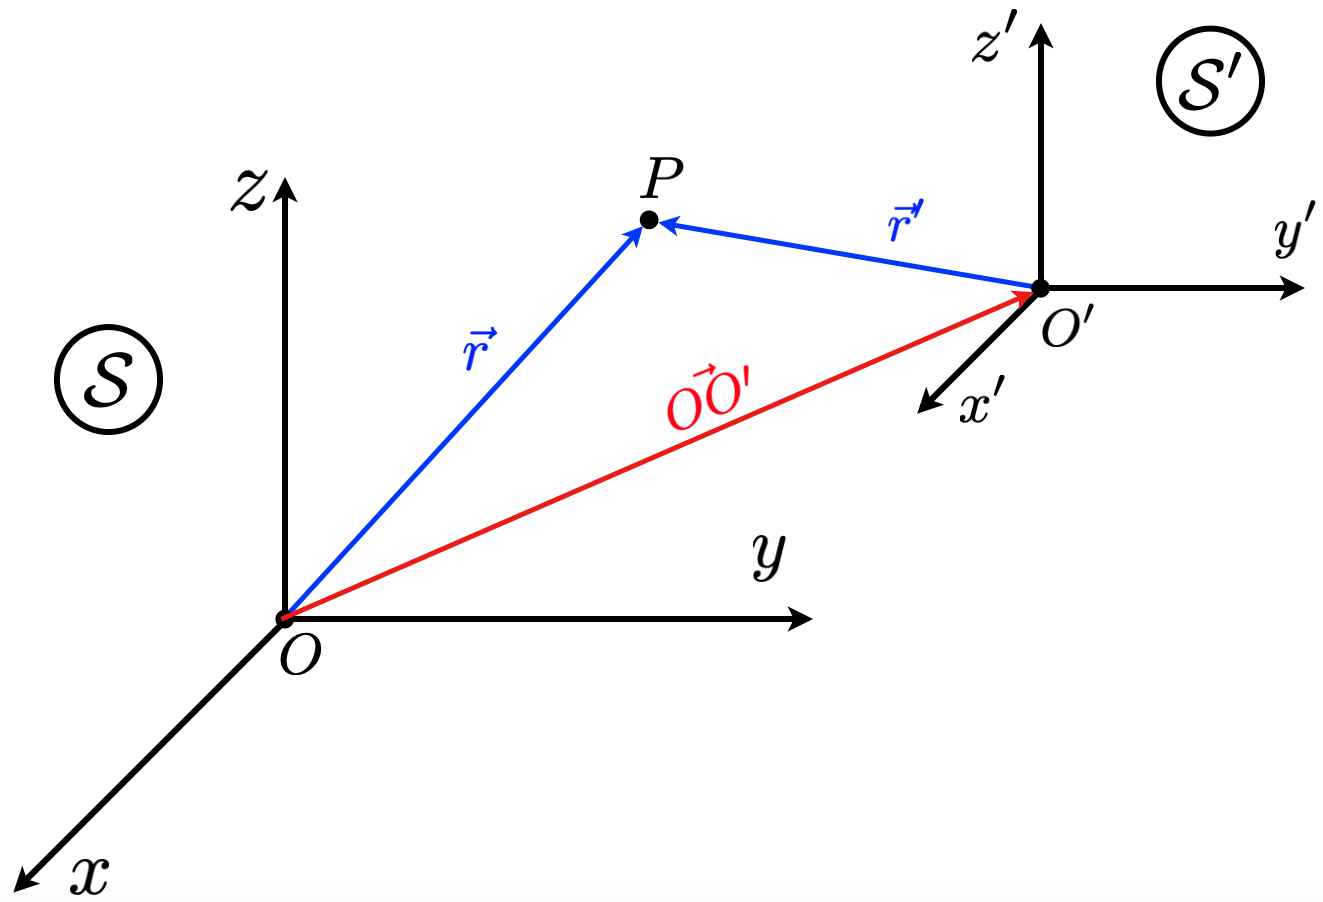
\includegraphics[width=10cm]{images/motirelativi.png}
\caption{Rappresentazione del sistema di riferimento fisso $\mathcal{S}$, e del sistema  $\mathcal{S'}$ in moto generico rispetto ad  $\mathcal{S}$.}
%\label{default}
\end{center}
\end{figure}

\section{Teorema delle velocità relative}

Dati due differenti sistemi di riferimento,  $\mathcal{S}$ in quiete, ed  $\mathcal{S'}$ in moto rispetto ad  $\mathcal{S}$, si vogliono trovare le relazioni che legano le grandezze osservate nel sistema fisso e quelle osservate nel sistema mobile.\\
Quindi preso un punto generico $P$ nello spazio, esso avrà come raggio vettore $\vec r$ in  $\mathcal{S}$, ed $\vec r'$ in  $\mathcal{S'}$.
\\Possiamo dunque scrivere che:

\begin{equation}
\vec r = \vec{OO'}+\vec r
\end{equation}

Dove $\vec{OO'}$ è il raggio vettore dell'origine del sistema $\mathcal{S'}$. Derivando rispetto al tempo l'equazione $(3.1)$ si otterrà la velocità del punto $P$ nel sistema $\mathcal{S}$ in funzione della velocità del punto $P$ in $\mathcal{S'}$, della velocità di traslazione del sistema $\mathcal{S'}$ ed in generale anche della velocità angolare con cui ruota $\mathcal{S'}$.

\begin{equation}
\boxed{\vec v = \vec v' + \vec u + \vec \omega\times\vec r'}
\end{equation}

\begin{equation}
\vec v_t \coloneqq \vec v - \vec v' = \vec u + \vec \omega\times\vec r'\seg \vec v = \vec v' + \vec v_t
\end{equation}
